\subsubsection{Trigonometrische Funktionen}
\begin{iequation}[align*]
	\tikz[remember picture] \coordinate(sinanchor) at (0,0); \sin x &= \sum_{n=0}^{\infty} \frac{(-1)^n x^{2n + 1}}{(2n+1)!} = x - \frac{x^3}{3!} + \frac{x^5}{5!}\ldots ~ \text{stetig}\\
	\tikz[remember picture] \coordinate(cosanchor) at (0,0); \cos x &= \sum_{n=0}^{\infty} \frac{(-1)^n x^{2n}}{(2n)!} = 1 - \frac{x^2}{2!} + \frac{x^4}{4!}\ldots \hspace{3.8mm} \text{stetig}\\
	\tan x &= \frac{\sin x}{\cos x} \hspace{10mm} \cot x = \frac{\cos x}{\sin x} \tikz[remember picture] \coordinate(trigfunkanchor) at (0,0);
\end{iequation}
\begin{tikzpicture}[remember picture, overlay]
	\node[overlaynote, text width = 28mm, anchor = west] at ($(trigfunkanchor) + (0.5,0.25)$) {$\pi$: kleinste strikt positive Nullstelle von $\sin$.};
	\node[overlaynote, rotate = 90] at ($(trigfunkanchor) + (3,2)$) {$\cos(x) = \sin \left(x + \frac{\pi}{2}\right)$};
	\node[overlaynote, rotate = 20, above left = 3mm and 2mm of sinanchor] (sinnote) {ungerade};
	\draw[overlayarrow] (sinnote) to[bend right] (sinanchor);
	\node[overlaynote, rotate = 20, above left = 3mm and 2mm of cosanchor] (cosnote) {gerade};
	\draw[overlayarrow] (cosnote) to[bend right] (cosanchor);
\end{tikzpicture}
\begin{comment}
\begin{flushleft}
    \begin{tikzpicture}[remember picture]
        \begin{axis} [
            samples=200,
            axis x line = middle,
            axis y line = left,
            grid = both,
            xtick={-pi,3*-pi/4,-pi/2,-pi/4,0,pi/4,pi/2,3*pi/4,pi,5*pi/4,3*pi/2,7*pi/4,2*pi},
            ytick={-1, -0.5, 0, 0.5, 1},
            xticklabels={$-\pi$, $-\frac{3\pi}{4}$, $-\frac{\pi}{2}$, $-\frac{\pi}{4}$, $0$,$\frac{\pi}{4}$,$\frac{\pi}{2}$,$\frac{3\pi}{4}$,$\pi$,$\frac{5\pi}{4}$,$\frac{3\pi}{2}$,$\frac{7\pi}{4}$,$2\pi$},
            width = 0.8\linewidth,
            height = 40mm,
            xmin=0,
            ymin=-1.2,
            xmax=6.5,
            ymax=1.2,
            legend entries = {$\sin(x)$, $\cos(x)$, $\tan(x)$},
            legend style = {
                anchor = north west, 
                font = \footnotesize,
            }
        ]
            \addplot[domain=0:6.28, darkblue, thick] {sin(deg(x))};
            \addplot[domain=0:6.28, darkred, thick] {cos(deg(x))};
            \addplot[domain=0:6.28, darkgreen, thick, opacity = 0.5] {tan(deg(x))};
            \pgfmathsetmacro\scyintersec{sin(deg(pi/4))}
            \coordinate(sincosintersec) at (axis cs: pi/4, \scyintersec);
        \end{axis}
    \end{tikzpicture}
    \tikz[remember picture, overlay] \node[draw= magenta!20, fill = none, semithick, circle, minimum size=3pt, inner sep = 0pt, outer sep = 0pt, pin={[pin edge={magenta!20, semithick}, draw = magenta!20, fill = magenta!20, rounded corners = 3pt]90:$\frac{4j + 1}{4} \cdot \pi | j \in \Z$}] at (sincosintersec) {};
\end{flushleft}
\begin{flushleft}
    \begin{tikzpicture}
        \begin{axis} [
            samples=400,
            axis x line = middle,
            axis y line = left,
            grid = both,
            xtick={-pi,3*-pi/4,-pi/2,-pi/4,0,pi/4,pi/2,3*pi/4,pi,5*pi/4,3*pi/2,7*pi/4,2*pi},
            ytick={-2, -1, -0.5, 0, 0.5, 1, 2},
            xticklabels={$-\pi$, $-\frac{3\pi}{4}$, $-\frac{\pi}{2}$, $-\frac{\pi}{4}$, $0$,$\frac{\pi}{4}$,$\frac{\pi}{2}$,$\frac{3\pi}{4}$,$\pi$,$\frac{5\pi}{4}$,$\frac{3\pi}{2}$,$\frac{7\pi}{4}$,$2\pi$},
            width = 0.8\linewidth,
            height = 40mm,
            xmin=0,
            ymin=-1.2,
            xmax=6.5,
            ymax=1.2,
            legend entries = {$\sin(x)$, $\sin(x)^2$, $\sin(x)^3$, $\sin(x^2)$, $\sin(\sin(x))$, $\cos(\cos(x))$},
            legend style = {
                anchor = north west, 
                font = \footnotesize,
            }
        ]
            \addplot[domain=0:6.28, opacity = 0.5] {sin(deg(x))};
            \addplot[domain=0:6.28, thick, mred] {sin(deg(x))^2};
            \addplot[domain=0:6.28, thick, darkblue] {sin(deg(x))^3};
            \addplot[domain=0:6.28, thick, opacity = 0.7, burntorange] {sin(deg(x^2))};
            \addplot[domain=0:6.28, thick, darkgreen] {sin(deg(sin(deg(x))))};
            \addplot[domain=0:6.28, thick, pastelaqua] {cos(deg(cos(deg(x))))};
        \end{axis}
    \end{tikzpicture}
\end{flushleft}
\end{comment}
 \begin{center}
    \renewcommand{\arraystretch}{1.3} %Zeilenabstand verändern
    \setlength{\tabcolsep}{4pt}
    \begin{tabular}{|c|c|c|c|c|c|c|c|c|c|}
        \hline
        Grad            & $0^\circ$ & $30^\circ$           & $45^\circ$           & $60^\circ$           & $90^\circ$      & $120^\circ$          & $135^\circ$           & $150^\circ$           & $180^\circ$ \\
        \hline
        $\varphi$       & $0$       & $\frac{\pi}{6}$      & $\frac{\pi}{4}$      & $\frac{\pi}{3}$      & $\frac{\pi}{2}$ & $\frac{2\pi}{3}$     & $\frac{3\pi}{4}$      & $\frac{5\pi}{6}$      & $\pi$       \\
        \hline
        $\sin(\varphi)$ & $0$       & $\frac{1}{2}$        & $\frac{\sqrt{2}}{2}$ & $\frac{\sqrt{3}}{2}$ & $1$             & $\frac{\sqrt{3}}{2}$ & $\frac{\sqrt{2}}{2}$  & $\frac{1}{2}$         & $0$         \\
        \hline
        $\cos(\varphi)$ & $1$       & $\frac{\sqrt{3}}{2}$ & $\frac{\sqrt{2}}{2}$ & $\frac{1}{2}$        & $0$             & $-\frac{1}{2}$       & $-\frac{\sqrt{2}}{2}$ & $-\frac{\sqrt{3}}{2}$ & $-1$        \\
        \hline
        $\tan(\varphi)$ & $0$       & $\frac{\sqrt{3}}{3}$ & $1$                  & $\sqrt{3}$           & $\pm \infty$    & -$\sqrt{3}$          & $-1$                  & $-\frac{\sqrt{3}}{3}$ & $0$         \\
        \hline
    \end{tabular}
\end{center}

\begin{theorem}{Eigenschaften sin/cos}
   \begin{enumerate}
       \item $\exp ix = \cos(x) + i \sin(x) \quad \forall x \in \mathbb{C}$
       \item $\cos x = \cos(-x) ~\text{und}~ \sin(-x) = -\sin x \quad\forall x \in \mathbb{C}$
       \item $\sin(x + y) = \sin(x)\cos(y) + \cos(x)\sin(y)$
       \item $\cos(x + y) = \cos(x)\cos(y) - \sin(x)\sin(y)$
       \item $\cos^2(x) + \sin^2(x) = 1 \quad \forall x \in \mathbb{C}$ 
       \item $\sin x = \frac{e^{iz} - e^{-iz}}{2i}, \quad \cos x = \frac{e^{iz} + e^{-iz}}{2}$
   \end{enumerate} 
\end{theorem}

\begin{corollary}{Winkelverdopplung}\\
        $\sin(2x) = 2 \sin(x)\cos(x)$ \hspace{4mm} $\cos(2x) = \cos^2(x) - \sin^2(x)$
\end{corollary}
\begin{corollary}{Potenz der Winkelfunktion}\\
    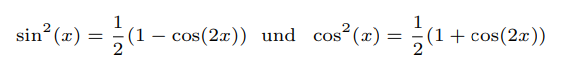
\includegraphics[scale=0.5]{Analysis1/zsf/Images/Basics/potenz_winkelfunktion.png}
\end{corollary}
\begin{corollary}{Eigenschaften mit $\pi$}
    \begin{enumerate}[itemsep= 2pt]
        \item $e^{i\pi} = -1, \quad e^{2i\pi} = 1$
        \item $\sin\left(x + \frac{\pi}{2}\right) = \cos(x), \quad \cos\left(x + \frac{\pi}{2}\right) = -\sin(x)$
        \item $\sin(x+\pi) = -\sin (x), \quad \sin(x + 2\pi) = \sin(x)$
        \item $\cos(x+\pi) = -\cos (x), \quad \cos(x + 2\pi) = \cos(x)$
    \end{enumerate}
\end{corollary}
\begin{corollary}{Nullstellen}
    \begin{enumerate}
         \item $\text{Nullstellen Sinus} = \{k\cdot \pi : k\in \mathbb{Z}\}$\\
        $\sin(x) > 0 \quad \forall x \in ]2k\pi, ~(2k+1)\pi[, ~ k\in \mathbb{Z}$\\[2pt]
        $\sin(x) < 0 \quad \forall x \in ](2k + 1)\pi, ~(2k+2)\pi[, ~ k\in \mathbb{Z}$
        \item $\text{Nullstellen Cosinus} = \left\{\frac{\pi}{2}+k\cdot \pi : k\in \mathbb{Z}\right\}$\\
        $\cos(x) > 0:\forall x \in \left]-\frac{\pi}{2} +2k\pi, ~-\frac{\pi}{2} +(2k+1)\pi\right[, ~ k\in \mathbb{Z}$\\[2pt]
        $\cos(x) < 0:\forall x \in \left]-\frac{\pi}{2} + (2k + 1)\pi, ~-\frac{\pi}{2} +(2k+2)\pi\right[, ~ k\in \mathbb{Z}$
    \end{enumerate}
\end{corollary}
\noindent Für $\tan(x)$ gilt $x \notin \frac{\pi}{2} + \pi \cdot \Z$ \qquad Für $\cot(x)$ gilt $x \notin \pi \Z$


